\documentclass [a4paper, 12pt] {article}
\usepackage{tikz}
\usepackage [margin = 3cm] {geometry}

\title{Data Structure}
\author{Pranto}
\date{\today}

\begin{document}

\maketitle

    \section{Graph 2}
    Lets make the graph of ED task 2.

    \vspace{20pt}
    \begin{center}
    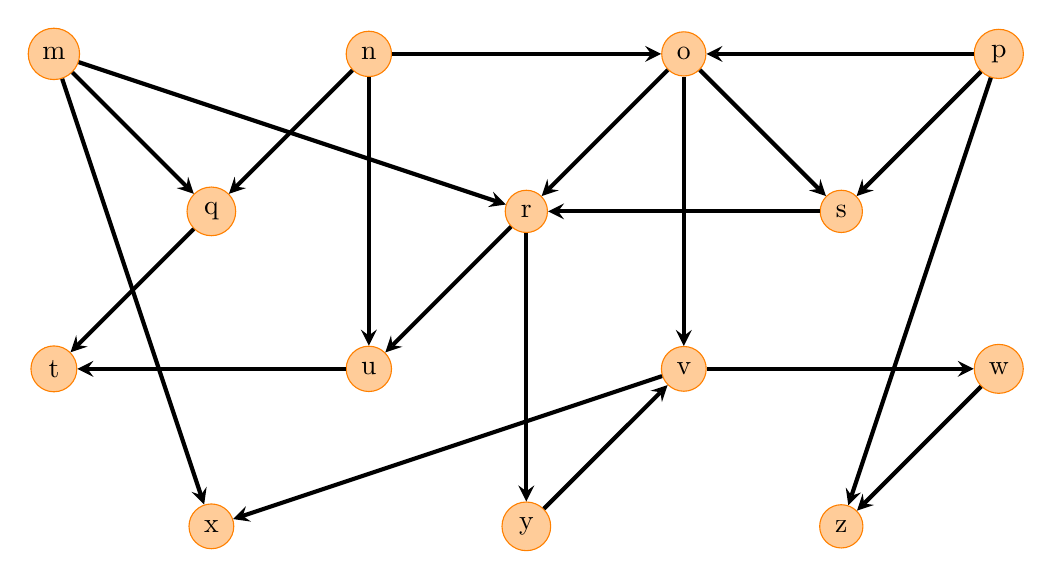
\begin{tikzpicture}
        % Nodes
        \node [draw = orange, fill = orange!40, circle] (m) at (0, 0) {m};
        \node [draw = orange, fill = orange!40, circle] (n) at (4, 0) {n};
        \node [draw = orange, fill = orange!40, circle] (o) at (8, 0) {o};
        \node [draw = orange, fill = orange!40, circle] (p) at (12, 0) {p};
        \node [draw = orange, fill = orange!40, circle] (q) at (2, -2) {q};
        \node [draw = orange, fill = orange!40, circle] (r) at (6, -2) {r};
        \node [draw = orange, fill = orange!40, circle] (s) at (10, -2) {s};
        \node [draw = orange, fill = orange!40, circle] (t) at (0, -4) {t};
        \node [draw = orange, fill = orange!40, circle] (u) at (4, -4) {u};
        \node [draw = orange, fill = orange!40, circle] (v) at (8, -4) {v};
        \node [draw = orange, fill = orange!40, circle] (w) at (12, -4) {w};
        \node [draw = orange, fill = orange!40, circle] (x) at (2, -6) {x};
        \node [draw = orange, fill = orange!40, circle] (y) at (6, -6) {y};
        \node [draw = orange, fill = orange!40, circle] (z) at (10, -6) {z};
        
        % Edges Direction
        \draw [->, > = stealth, line width = 1.5pt] (m) -- (q);
        \draw [->, > = stealth, line width = 1.5pt] (m) -- (x);
        \draw [->, > = stealth, line width = 1.5pt] (m) -- (r);
        \draw [->, > = stealth, line width = 1.5pt] (n) -- (o);
        \draw [->, > = stealth, line width = 1.5pt] (p) -- (o);
        \draw [->, > = stealth, line width = 1.5pt] (n) -- (q);
        \draw [->, > = stealth, line width = 1.5pt] (n) -- (u);
        \draw [->, > = stealth, line width = 1.5pt] (o) -- (r);
        \draw [->, > = stealth, line width = 1.5pt] (o) -- (v);
        \draw [->, > = stealth, line width = 1.5pt] (o) -- (s);
        \draw [->, > = stealth, line width = 1.5pt] (p) -- (s);
        \draw [->, > = stealth, line width = 1.5pt] (p) -- (z);
        \draw [->, > = stealth, line width = 1.5pt] (q) -- (t);
        \draw [->, > = stealth, line width = 1.5pt] (r) -- (u);
        \draw [->, > = stealth, line width = 1.5pt] (r) -- (y);
        \draw [->, > = stealth, line width = 1.5pt] (s) -- (r);
        \draw [->, > = stealth, line width = 1.5pt] (u) -- (t);
        \draw [->, > = stealth, line width = 1.5pt] (v) -- (x);
        \draw [->, > = stealth, line width = 1.5pt] (v) -- (w);
        \draw [->, > = stealth, line width = 1.5pt] (w) -- (z);
        \draw [->, > = stealth, line width = 1.5pt] (y) -- (v);

    \end{tikzpicture}
\end{center}
\end{document}